\documentclass[a4paper,10pt]{article}
\usepackage[utf8]{inputenc}
\usepackage{amsmath}
\usepackage[pdftex]{graphicx}
\usepackage{fullpage}
\usepackage{listings}
\usepackage{amssymb}
\usepackage{url}

\title{\textbf{CSC2515 Project Proposal} \\
Autonomous Driving: Road-Estimation}
\author{
  Jacob Lambert\footnote{jacob.lambert@mail.utoronto.ca}~~(1001319842)\\
  Rikky Duivenvoorden\footnote{rikky.duivenvoorden@mail.utoronto.ca}~~(997455329) \\
}
\date{}

\pdfinfo{%
  /Title    (CSC2515 Project Proposal)
  /Author   (Jacob Lambert and Rikky Duivenvoorden)
  /Creator  ()				
  /Producer ()
  /Subject  (Machine Learning)
  /Keywords ()
}

\begin{document}
\maketitle

\section{Project Overview}
The project we propose consists of a comparison of classification algorithms in their ability to accurately classsify what is road and non-road in the suggested autonomous driving: road estimation topic. The dataset is the base kit of the road/lane detection evaluation of the KITTI dataset, described in further detail below. The training data will be split into 60\% for training, 10\% for validation, and 30\% for testing, and preprocessed to conduct the classification on superpixels. The algorithms used for comparison are listed below, and will be compared in false-positive and false-negative error rates.


\section{Dataset}
The data used in this project is provided by the KITTI Vision Benchmarking Suite\footnote{ \url{http://www.cvlibs.net/datasets/kitti/}} which is widely used in robotics for testing machine learning algorithms. The Road/Lane Detection Evaluation (2013) dataset contains images (pixel color intensity) of urban scenes taken from the top of a vehicle, which ground truth labels for roads. There are three different scene categories, as seen in figure \ref{fig:kitti}:
\begin{itemize}
 \item urban unmarked roads (uu),
 \item urban marked roads (um),
 \item urban roads with multiple marked lanes (umm),
\end{itemize}
each with roughly 100 training images and 100 test images.
\begin{figure}[ht!]
 \centering
 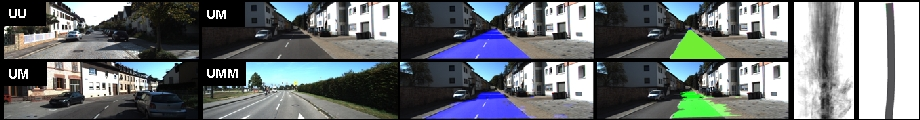
\includegraphics[width=0.99\textwidth]{figs/kitti.jpg}
 \caption{Example of the different scenes in this KITTI dataset with road labels.}\label{fig:kitti}
\end{figure}
The main dataset used will be the urban marked road dataset as project focuses road estimation and not individual lanes. A possible extension to this project would be to analyze the impact of scene type by evaluating performance on all datasets individually, then combining them.

\section{Algorithms}
This project will compare three supervised learning algorithms and potentially a state-of-the-art technique. The three benchmarking algorithms are:
\begin{description}
 \item[Regression], relates input and output based on a function. Several different functions will be tested (linear, logistic, polynomial).
 \item[$k$NN], which classifies based on the majority vote of its $k$ Nearest Neighbours in feature space.
 \item[Support Vector Machines (SVM)], which attempts to learn a map from the input to a seperable feature space used for classification.
\end{description}

There are several possibilities for state-of-the-art techniques to test for this task. An obvious choice would be Convoluted Neural Networks which, according to the KITTI leaderboard, perform very well on this task\cite{}. Further research will be required to find a complex algorithm that remains within the scope of this course.

\section{References}

\end{document}
